\section{模块设计}

\par 综上所述,拟将系统划分为八个模块:数据采集模块、位姿估计与场景管理模块、数据预处理与语义分割模块、点云生成与语义融合模块、可视化模块、点云后处理模块、模型导入导出模块和用户管理模块。
系统总体功能结构图如图\ref{fig:function}所示。

\begin{figure}[htb]
	\centering
	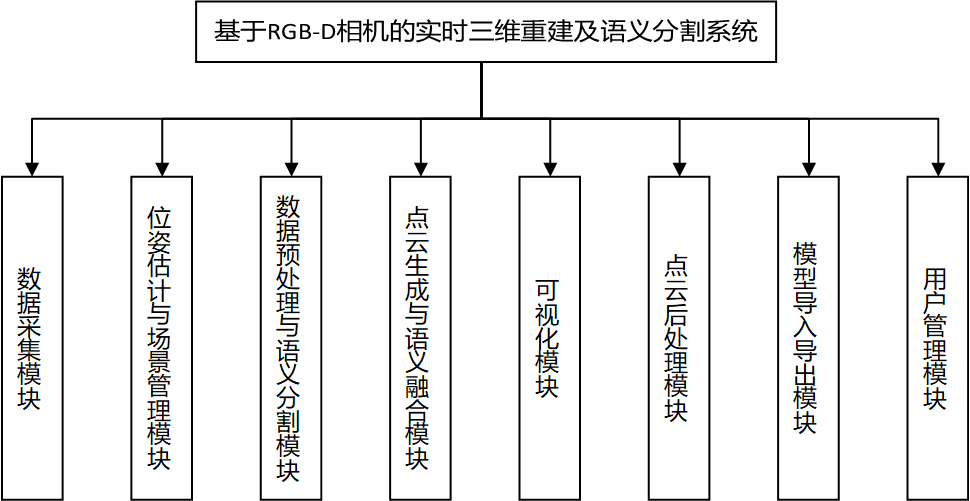
\includegraphics[width=0.9\textwidth]{figures/uml/function_all.png}
	\caption{系统功能结构图}
	\label{fig:function}
\end{figure}

\subsection{数据采集模块}
\par 该模块的主要任务是管理和控制RGB-D相机,捕获并处理来自RGB-D相机的图像数据,包括RGB图像,深度图像和语义分割图像,涉及到使用相机制造商提供的SDK,活动图如图\ref{fig:activity1}所示。模块包含以下功能:

\begin{enumerate}
	\item{相机接口}
	\par 使用Intel RealSense相机进行数据采集,通过Intel RealSense SDK 2.0进行通信。相机接口需要实现启动、停止、设定参数、获取数据等功能,以便在系统中灵活地控制相机。

	\item{图像格式转换}
	\par 将相机获取的原始图像数据转换成RGB格式,以满足系统的需求。转换过程中需要确保图像数据的正确性和完整性。

	\item{时间戳同步}
	\par 为了确保RGB图像和深度图像的一致性,需要对它们的时间戳进行同步。同步方法包括硬件同步和软件同步。硬件同步需要相机支持,而软件同步则需要在系统中实现。同步方法可以根据实际需求和相机性能选择。

	\item{缓冲区管理}
	\par 为了解决数据采集速率与数据处理速率的不匹配问题,需要实现缓冲区管理。采用循环缓冲区策略,为RGB图像和深度图像分别分配一定数量的缓冲区。当缓冲区满时,系统自动覆盖最旧的数据,确保实时性。缓冲区管理需要考虑数据读写的并发性和同步问题。

	\item{数据流控制}
	\par 数据流控制负责在数据采集和处理过程中协调各个模块之间的数据传递。数据流控制需要确保数据的有效性、完整性和正确性,同时考虑各模块的处理速度和系统的实时性。

	\item{异常处理与容错}
	\par 该模块需要具备异常处理与容错功能,以应对硬件故障、通信中断、数据丢失等问题。异常处理机制包括超时检测、重试策略、数据恢复等。容错功能可以通过冗余设计、备份策略等方法实现。
\end{enumerate}

\par 通过实现这些功能,可以确保系统有效地从RGB-D相机获取RGB图像和深度图像,并在后续模块中进行处理和分析。

\begin{figure}[htb]
	\centering
	\begin{minipage}[t]{0.45\linewidth}
		\centering
		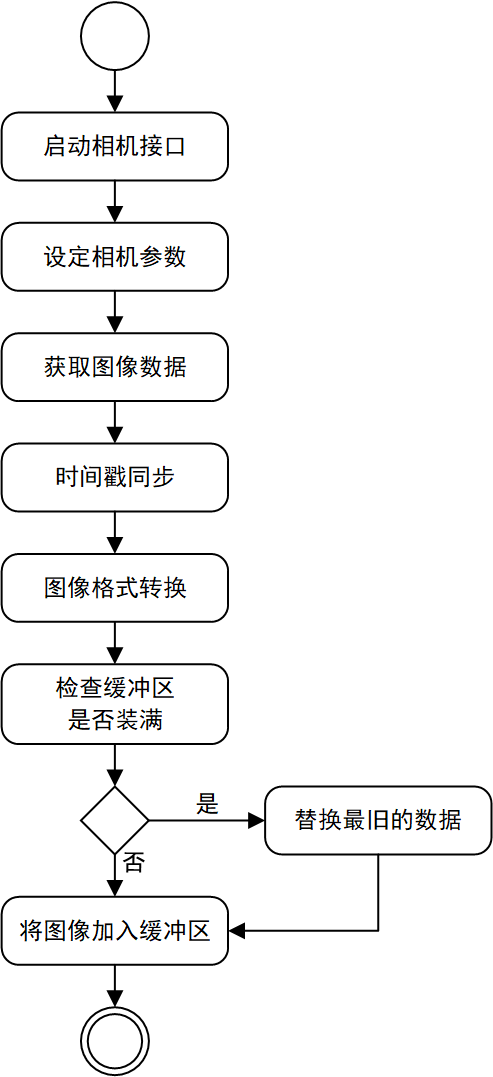
\includegraphics[height=12cm,keepaspectratio]{figures/uml/activity1.png}
		\caption{数据采集模块活动图}
		\label{fig:activity1}
	\end{minipage}
	\begin{minipage}[t]{0.45\linewidth}
		\centering
		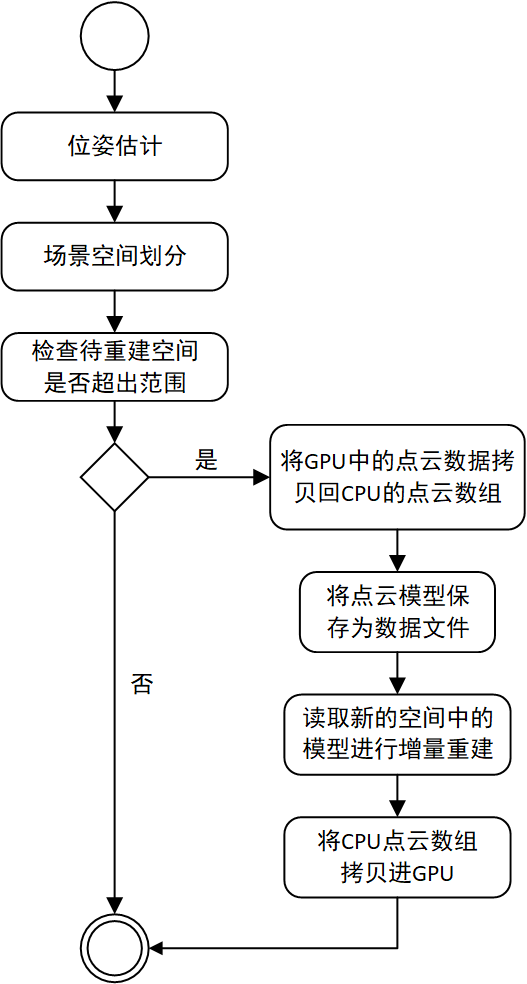
\includegraphics[height=12cm,keepaspectratio]{figures/uml/activity2.png}
		\caption{位姿估计与场景管理模块活动图}
		\label{fig:activity2}
	\end{minipage}
\end{figure}

\subsection{位姿估计与场景管理模块}
\par 该模块负责根据连续的RGB图像和深度图像计算相机的位姿矩阵,以及场景空间划分和重建范围判断,以便在有限的资源下进行重建。如图\ref{fig:activity2}所示,该模块连接并协调数据采集模块与后续处理模块,起着至关重要的作用,包含以下功能:
\begin{enumerate}
	\item{位姿估计}
	\par 使用对极几何算法,根据连续的RGB图像和深度图像计算其对应的位姿矩阵。位姿矩阵的计算结果将对点云模型的精度产生重要影响,需要确保计算结果的实时性和准确性。

	\item{场景空间划分}
	\par 将整个场景空间分成若干空间网格。由于网格位置是固定的,为避免相机移动到网格边缘时,捕捉到网格外的信息,产生数据丢失,可以将空间划分为四分之一重叠空间网格(Quarter-Overlapping Spatial Grid)\cite{CompressibleLES}。需要根据实际场景和内存限制选择合适的网格参数。

	\item{重建范围判断与场景更新}
	\par 空间划分完成后,根据相机位姿矩阵,判断新的待重建空间是否超出了范围。如果超出了范围,则先将GPU中的点云数据拷贝回CPU的点云数组中,调用模型导入导出模块,根据坐标位置将点云模型保存为数据文件。然后读取新的空间中的模型进行增量重建。

	\item{数据交换与管理}
	\par 实现CPU与GPU之间的数据交换与管理,需要考虑处理速度、资源竞争和系统稳定性等因素。
\end{enumerate}

\subsection{数据预处理与语义分割模块}
\par 该模块负责对捕获的RGB图像和深度图像进行预处理,并使用深度学习方法对RGB图像进行语义分割,活动图如图\ref{fig:activity3}所示。模块包含以下功能:

\begin{enumerate}
	\item{RGB图像与深度图像对齐}
	\par 使用Intel RealSense相机内参、RGB图像和深度图像的位姿矩阵,将RGB图像和深度图像进行对齐。这样可以确保在后续的语义分割和三维重建过程中,像素点的对应关系是准确的。对齐过程需要考虑相机内参、畸变等因素,以获得准确的对齐结果。

	\item{语义分割}
	\par 使用kMaX-DeepLab模型对RGB图像进行语义分割,为每个像素匹配一个语义类别标签。首先需要选择合适的预训练模型,然后根据实际应用场景对模型进行微调,以实现高效准确的分割。在此过程中,可以利用深度图像提供的距离信息进行辅助,提高分割准确性。

	\item{图像去噪与增强}
	\par 使用中值滤波、高斯滤波等技术对图像进行去噪操作,提高图像的可识别性。

	\item{无效区域裁剪与缩放}
	\par 根据相机的视场范围和测量范围,对图像进行裁剪,去除无效区域(如遮挡、边缘等),并将图像缩放至系统规定尺寸,这有助于缓解后续TSDF算法产生的拖尾现象(Ghosting Artefacts),提高处理的效率和质量。此步骤需要确保缩放后的图像不影响三维重建的精度。

	\item{图像格式转换与数值归一化}
	\par 将图像格式转换成系统规定格式(如大小端、数据类型等),并且进行归一化,使得每个像素的值在0到1之间。
\end{enumerate}

\par 通过这一系列的操作,该模块可以有效地对每一帧图像进行处理,为后续的点云生成以及可视化等
操作提供高质量的输入,不仅提高了整个系统的准确性,也提高了系统的实时性。

\begin{figure}[htb]
	\centering
	\begin{minipage}[t]{0.45\linewidth}
		\centering
		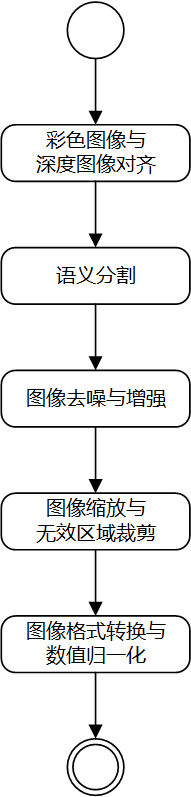
\includegraphics[height=12cm,keepaspectratio]{figures/uml/activity3.png}
		\captionsetup{justification=centering}
		\caption{数据预处理语义分割模块活动图}
		\label{fig:activity3}
	\end{minipage}
	\begin{minipage}[t]{0.45\linewidth}
		\centering
		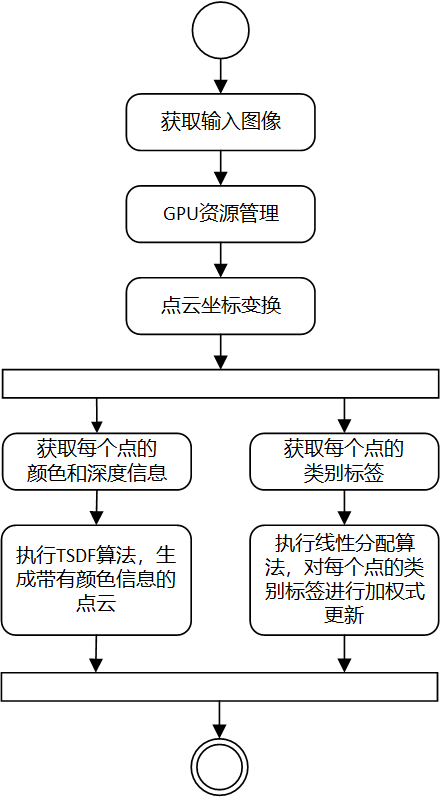
\includegraphics[height=12cm,keepaspectratio]{figures/uml/activity4.png}
		\captionsetup{justification=centering}
		\caption{点云生成与语义融合模块活动图}
		\label{fig:activity4}
	\end{minipage}
\end{figure}

\subsection{点云生成与语义融合模块}
\par 该模块是系统的核心模块,负责根据RGB图像、深度图像、语义分割图像和相机位姿生成点云数据,实时地对点云数据中的类别标签进行融合与更新,并确保生成的三维模型在几何和语义上保持一致,活动图如图\ref{fig:activity4}所示。模块包含以下功能:
\begin{enumerate}
	\item{GPU资源管理}
	\par 由于点云生成涉及大量的矩阵运算,因此使用GPU进行TSDF算法的加速计算,可以提高点云生成效率。该模块的计算任务将在GPU上执行,其中涉及GPU内存的分配和回收,以及GPU线程分配方案的设计。

	\item{实时点云生成}
	\par 在收到输入数据后,首先根据相机内参和相机位姿进行坐标变换,通过该点在世界坐标系中的坐标计算出相机坐标中的坐标,判断该点是否与RGB图像中的某个像素匹配。其次,执行TSDF算法,通过与RGB图像和深度图像的对比,判断该点是否属于图像中的某个物体。若属于某个物体,则将该点的RGB值与对应像素的RGB值关联,生成带有RGB信息的点云。

	\item{实时语义融合与更新}
	\par 生成点云数据后,对点云进行语义融合。首先,通过与获取RGB值类似的方法,将点云坐标映射到语义分割图像上,获取每个点的类别标签。然后,使用线性分配方法对每个点的类别标签进行更新。为了确保实时性,同样可以使用GPU加速计算。
\end{enumerate}

\par 通过以上步骤,可以实现高效、准确的点云生成与语义融合,为整个三维重建及语义分割系统提供核心支持。整个过程需要考虑数据结构的设计、算法的高效实现以及多线程任务调度和资源管理,具有一定的挑战性。

\subsection{可视化模块}
\par 该模块提供了对于整个系统输出的直观展示,对系统开发及用户体验起着至关重要的作用。模块需要提供友好的交互功能和实时的图形用户界面,以便用户查看和分析重建的三维模型,活动图如图\ref{fig:activity5}所示。模块包含以下功能:

\begin{enumerate}
	\item{窗口管理}
	\par 负责创建和管理两个独立的窗口,一个用于显示RGB动画,另一个用于显示语义动画。使用GLFW处理窗口创建和输入事件。支持窗口大小调整、全屏切换等功能。

	\item{实时渲染引擎}
	\par 使用OpenGL开发一个实时渲染引擎,负责实现渲染管线、显示点云数据、相机位姿以及其他相关信息。其中,渲染管线包括顶点着色器和片段着色器。为了实现不同的颜色和效果,需要为RGB动画和语义动画分别设置不同的着色器程序。此外,渲染引擎应支持渲染不同类型的几何数据(例如点、线、三角形等),以及实时更新渲染内容。

	\item{数据传输}
	\par 负责从点云生成与语义融合模块获取实时数据,将数据传递给实时渲染引擎进行绘制。为了实现实时可视化,需要使用双缓冲技术,将新生成的点云数据传输到OpenGL的缓冲区\texttt{VBO}中,同时确保不影响渲染性能。

	\item{交互控制}
	\par 负责处理用户输入,例如缩放、旋转和平移视图。可以使用鼠标和键盘事件来实现这些功能,根据用户操作调整相机参数。

	\item{动画同步}
	\par 负责同步更新RGB动画和语义动画,可以使用OpenGL的时间戳功能实现动画的同步,并根据系统的实时性能自动调整动画速度。

	\item{性能优化(可选)}
	\par 为了提升实时可视化的流畅性,可以对渲染性能进行优化。这包括合理地调整渲染质量与速度之间的平衡、使用多线程技术并行处理数据以及使用GPU加速渲染等。
\end{enumerate}

\par 可视化模块将复杂的点云数据和语义信息转换为直观的二维图像,以便用户理解和分析。该模块的实现主要依赖于OpenGL和GLFW等图形库和高效的数据传输和实时渲染技术。

\begin{figure}[htb]
	\centering
	\begin{minipage}[t]{0.45\linewidth}
		\centering
		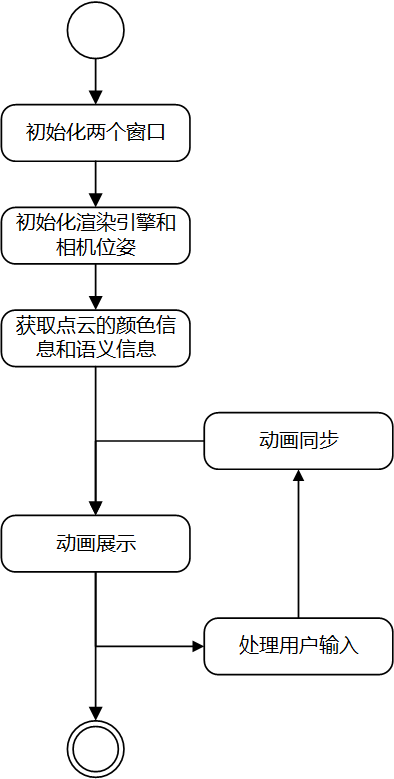
\includegraphics[height=12cm,keepaspectratio]{figures/uml/activity5.png}
		\caption{可视化模块活动图}
		\label{fig:activity5}
	\end{minipage}
	\begin{minipage}[t]{0.45\linewidth}
		\centering
		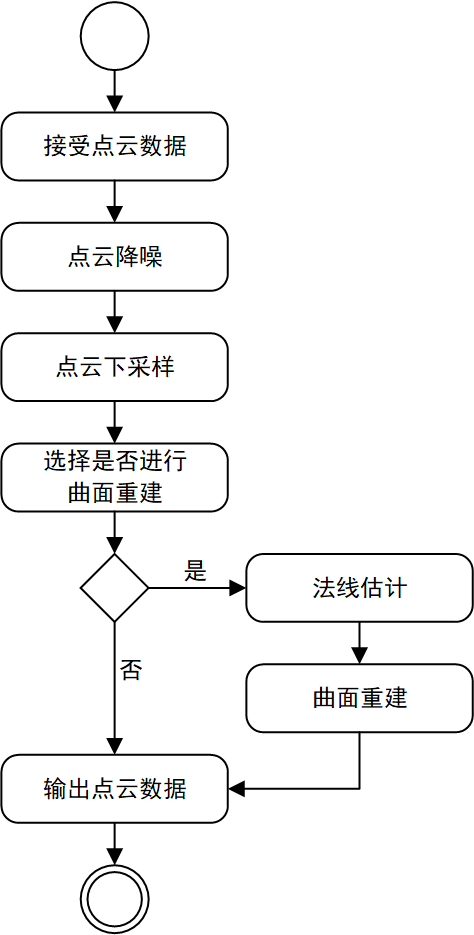
\includegraphics[height=12cm,keepaspectratio]{figures/uml/activity6.png}
		\caption{点云后处理模块活动图}
		\label{fig:activity6}
	\end{minipage}
\end{figure}

\subsection{点云后处理模块}
\par 该模块是三维重建及语义分割系统的重要组成部分,负责对融合后的点云进行优化和滤波处理,提高模型质量和精度。同时,也提供了一些可选的高级功能,如点云下采样、表面法线估
计和曲面重建,生成表面更连续的模型,活动图如图\ref{fig:activity6}所示。该模块包含以下功能:
\begin{enumerate}
	\item{点云降噪}
	\par 在室内重建中,基于局部密度的滤波在去除噪声的同时能够保留边缘信息。因此,选用基于局部密度的滤波对点云数据进行降噪操作,移除离群点和噪声点。

	\item{点云下采样(可选)}
	\par 使用八叉树结构对点云数据进行下采样,可以减少点云数量并降低计算和存储成本,同时最大程度保留点云的整体结构。

	\item{法线估计(可选)}
	\par 基于邻域点集为每个点计算表面法线,以便在曲面重建中使用。常用的法线估计方法包括主成分分析(Principal Component Analysis,PCA)、近邻搜索和法线一致性等方法。

	\item{曲面重建(可选)}
	\par 根据优化后的点云生成平滑、连续的三维表面模型。可采用的算法包括贪婪投影三角化、泊松重建、球形重建等。
\end{enumerate}

\par 为了实现可选的功能,可以使用Open3D点云处理库进行开发。通过Open3D提供的点云处理和曲面重建功能,可以高效地实现模块的需求。

\subsection{模型导入导出模块}
\par 该模块主要负责管理和转换三维点云模型的输入输出,一般由其他模块调用,实现灵活地导入和导出三维模型。该模块使用PLY作为点云模型的存储格式,并确保语义信息与模型一起导入导出,活动图如图\ref{fig:activity7}所示。模块包含以下功能:

% \begin{figure}[htb]
% 	\centering
% 	\includegraphics[height=12cm,keepaspectratio]{figures/uml/activity7.png}
% 	\caption{模型导入导出模块活动图}
% 	\label{fig:activity7}
% \end{figure}

\begin{figure}[htbp]
	\centering
	\subfigure[模型导入]{
		\begin{minipage}[t]{0.48\linewidth}
			\centering
			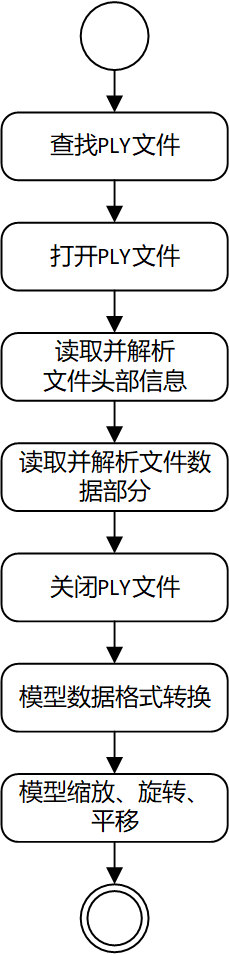
\includegraphics[height=12cm,keepaspectratio]{figures/uml/activity7_1.png}
		\end{minipage}
	}
	\subfigure[模型导出]{
		\begin{minipage}[t]{0.48\linewidth}
			\centering
			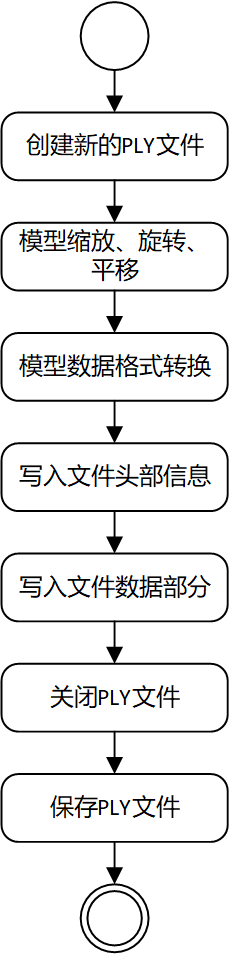
\includegraphics[height=12cm,keepaspectratio]{figures/uml/activity7_2.png}
		\end{minipage}
	}
	\caption{模型导入导出模块活动图}
	\label{fig:activity7}
\end{figure}

\begin{enumerate}
	\item{文件读取与解析}
	\par 设计一个文件读取接口,负责读取和解析PLY文件中的几何信息和语义信息,包括打开文件、读取文件和关闭文件等基本操作。接口需要实现解析PLY文件头部的功能,以获取顶点数量、属性信息等;同时,还需解析文件数据部分,以提取顶点坐标、颜色、类别标签等信息。在解析过程中,需要处理不同的数据类型(如ASCII和Binary)以及不同的属性值。

	\item{数据格式转换}
	\par 将解析得到的几何信息和语义信息转换为系统使用的数据格式,例如点云结构体数组。同时,支持将系统使用的数据格式转换为导出时所需的几何信息和语义信息。

	\item{模型信息同步}
	\par 实现模型的缩放、旋转、平移等变换操作,以确保导入模型信息与当前模型保持一致。这些操作应该能够在内部数据格式上直接进行,避免重复的格式转换。

	\item{文件写入与导出}
	\par 设计一个文件写入接口,负责将点云模型写入PLY文件,包括创建新文件、写入文件和关闭文件等基本操作。与文件读取相似,同样需要实现写入PLY文件头部以及文件数据部分。
\end{enumerate}

\subsection{用户管理模块}
\par 该模块负责管理系统中的用户,包括权限、注册、登录、删除和角色管理功能,目标是确保系统的安全性和合规性,活动图如图\ref{fig:activity8}所示。模块包含以下功能:

\begin{figure}[htb]
	\centering
	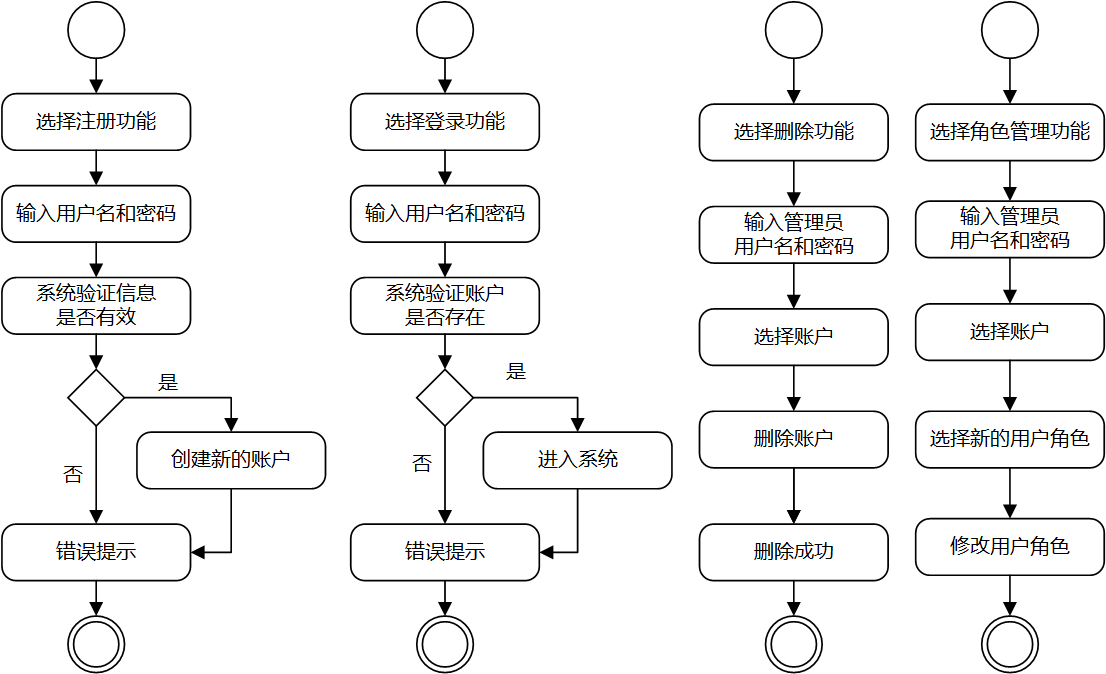
\includegraphics[width=1\textwidth]{figures/uml/activity8.png}
	\caption{用户管理模块活动图}
	\label{fig:activity8}
\end{figure}

\begin{enumerate}
	\item{用户注册}
	\par 用户可以通过该功能注册系统账户。在注册时,用户需要提供必要的个人信息,并创建一个安全的登录凭证(用户名和密码)。系统将验证用户提供的信息,确保注册信息的准确性和安全性。一旦注册成功,用户将获得系统的访问权限。
	
	\item{用户登录}
	\par 已注册的用户可以登录系统。用户需要提供其注册时创建的用户名和密码进行身份验证。登录后,用户将能够访问系统的功能和数据。
	
	\item{用户删除}
	\par 允许管理员删除用户账户,以确保只有授权用户能够访问系统功能和数据。删除账户后,用户将失去对系统的访问权限,并且其个人信息将被移除。
	
	\item{角色管理}
	\par 系统中的用户分为不同的角色,包括系统操作员、数据工程师、算法研究员和项目决策者。管理员可以为每个用户分配适当的角色,以确保他们只能访问与其工作职责相关的功能和数据。
\end{enumerate}

\par 用户管理模块需要确保用户对系统的安全使用和适当的权限管理,这对于系统的运行稳定性和生成结果质量至关重要。